% Options for packages loaded elsewhere
\PassOptionsToPackage{unicode}{hyperref}
\PassOptionsToPackage{hyphens}{url}
\PassOptionsToPackage{dvipsnames,svgnames,x11names}{xcolor}
%
\documentclass[
  letterpaper,
  DIV=11,
  numbers=noendperiod]{scrartcl}

\usepackage{amsmath,amssymb}
\usepackage{iftex}
\ifPDFTeX
  \usepackage[T1]{fontenc}
  \usepackage[utf8]{inputenc}
  \usepackage{textcomp} % provide euro and other symbols
\else % if luatex or xetex
  \usepackage{unicode-math}
  \defaultfontfeatures{Scale=MatchLowercase}
  \defaultfontfeatures[\rmfamily]{Ligatures=TeX,Scale=1}
\fi
\usepackage{lmodern}
\ifPDFTeX\else  
    % xetex/luatex font selection
\fi
% Use upquote if available, for straight quotes in verbatim environments
\IfFileExists{upquote.sty}{\usepackage{upquote}}{}
\IfFileExists{microtype.sty}{% use microtype if available
  \usepackage[]{microtype}
  \UseMicrotypeSet[protrusion]{basicmath} % disable protrusion for tt fonts
}{}
\makeatletter
\@ifundefined{KOMAClassName}{% if non-KOMA class
  \IfFileExists{parskip.sty}{%
    \usepackage{parskip}
  }{% else
    \setlength{\parindent}{0pt}
    \setlength{\parskip}{6pt plus 2pt minus 1pt}}
}{% if KOMA class
  \KOMAoptions{parskip=half}}
\makeatother
\usepackage{xcolor}
\setlength{\emergencystretch}{3em} % prevent overfull lines
\setcounter{secnumdepth}{5}
% Make \paragraph and \subparagraph free-standing
\makeatletter
\ifx\paragraph\undefined\else
  \let\oldparagraph\paragraph
  \renewcommand{\paragraph}{
    \@ifstar
      \xxxParagraphStar
      \xxxParagraphNoStar
  }
  \newcommand{\xxxParagraphStar}[1]{\oldparagraph*{#1}\mbox{}}
  \newcommand{\xxxParagraphNoStar}[1]{\oldparagraph{#1}\mbox{}}
\fi
\ifx\subparagraph\undefined\else
  \let\oldsubparagraph\subparagraph
  \renewcommand{\subparagraph}{
    \@ifstar
      \xxxSubParagraphStar
      \xxxSubParagraphNoStar
  }
  \newcommand{\xxxSubParagraphStar}[1]{\oldsubparagraph*{#1}\mbox{}}
  \newcommand{\xxxSubParagraphNoStar}[1]{\oldsubparagraph{#1}\mbox{}}
\fi
\makeatother


\providecommand{\tightlist}{%
  \setlength{\itemsep}{0pt}\setlength{\parskip}{0pt}}\usepackage{longtable,booktabs,array}
\usepackage{calc} % for calculating minipage widths
% Correct order of tables after \paragraph or \subparagraph
\usepackage{etoolbox}
\makeatletter
\patchcmd\longtable{\par}{\if@noskipsec\mbox{}\fi\par}{}{}
\makeatother
% Allow footnotes in longtable head/foot
\IfFileExists{footnotehyper.sty}{\usepackage{footnotehyper}}{\usepackage{footnote}}
\makesavenoteenv{longtable}
\usepackage{graphicx}
\makeatletter
\newsavebox\pandoc@box
\newcommand*\pandocbounded[1]{% scales image to fit in text height/width
  \sbox\pandoc@box{#1}%
  \Gscale@div\@tempa{\textheight}{\dimexpr\ht\pandoc@box+\dp\pandoc@box\relax}%
  \Gscale@div\@tempb{\linewidth}{\wd\pandoc@box}%
  \ifdim\@tempb\p@<\@tempa\p@\let\@tempa\@tempb\fi% select the smaller of both
  \ifdim\@tempa\p@<\p@\scalebox{\@tempa}{\usebox\pandoc@box}%
  \else\usebox{\pandoc@box}%
  \fi%
}
% Set default figure placement to htbp
\def\fps@figure{htbp}
\makeatother
% definitions for citeproc citations
\NewDocumentCommand\citeproctext{}{}
\NewDocumentCommand\citeproc{mm}{%
  \begingroup\def\citeproctext{#2}\cite{#1}\endgroup}
\makeatletter
 % allow citations to break across lines
 \let\@cite@ofmt\@firstofone
 % avoid brackets around text for \cite:
 \def\@biblabel#1{}
 \def\@cite#1#2{{#1\if@tempswa , #2\fi}}
\makeatother
\newlength{\cslhangindent}
\setlength{\cslhangindent}{1.5em}
\newlength{\csllabelwidth}
\setlength{\csllabelwidth}{3em}
\newenvironment{CSLReferences}[2] % #1 hanging-indent, #2 entry-spacing
 {\begin{list}{}{%
  \setlength{\itemindent}{0pt}
  \setlength{\leftmargin}{0pt}
  \setlength{\parsep}{0pt}
  % turn on hanging indent if param 1 is 1
  \ifodd #1
   \setlength{\leftmargin}{\cslhangindent}
   \setlength{\itemindent}{-1\cslhangindent}
  \fi
  % set entry spacing
  \setlength{\itemsep}{#2\baselineskip}}}
 {\end{list}}
\usepackage{calc}
\newcommand{\CSLBlock}[1]{\hfill\break\parbox[t]{\linewidth}{\strut\ignorespaces#1\strut}}
\newcommand{\CSLLeftMargin}[1]{\parbox[t]{\csllabelwidth}{\strut#1\strut}}
\newcommand{\CSLRightInline}[1]{\parbox[t]{\linewidth - \csllabelwidth}{\strut#1\strut}}
\newcommand{\CSLIndent}[1]{\hspace{\cslhangindent}#1}

\KOMAoption{captions}{tableheading}
\makeatletter
\@ifpackageloaded{caption}{}{\usepackage{caption}}
\AtBeginDocument{%
\ifdefined\contentsname
  \renewcommand*\contentsname{Table of contents}
\else
  \newcommand\contentsname{Table of contents}
\fi
\ifdefined\listfigurename
  \renewcommand*\listfigurename{List of Figures}
\else
  \newcommand\listfigurename{List of Figures}
\fi
\ifdefined\listtablename
  \renewcommand*\listtablename{List of Tables}
\else
  \newcommand\listtablename{List of Tables}
\fi
\ifdefined\figurename
  \renewcommand*\figurename{Figure}
\else
  \newcommand\figurename{Figure}
\fi
\ifdefined\tablename
  \renewcommand*\tablename{Table}
\else
  \newcommand\tablename{Table}
\fi
}
\@ifpackageloaded{float}{}{\usepackage{float}}
\floatstyle{ruled}
\@ifundefined{c@chapter}{\newfloat{codelisting}{h}{lop}}{\newfloat{codelisting}{h}{lop}[chapter]}
\floatname{codelisting}{Listing}
\newcommand*\listoflistings{\listof{codelisting}{List of Listings}}
\makeatother
\makeatletter
\makeatother
\makeatletter
\@ifpackageloaded{caption}{}{\usepackage{caption}}
\@ifpackageloaded{subcaption}{}{\usepackage{subcaption}}
\makeatother

\usepackage{bookmark}

\IfFileExists{xurl.sty}{\usepackage{xurl}}{} % add URL line breaks if available
\urlstyle{same} % disable monospaced font for URLs
\hypersetup{
  pdftitle={DISCOV-Gracilaria Paper},
  pdfauthor={Simon Oiry¹; Bede Ffinian Rowe Davies¹; Pierre Gernez¹; Laurent Barillé¹},
  pdfkeywords={Remote Sensing, Invasive species, Coastal
Ecosystems, Biodiversity},
  colorlinks=true,
  linkcolor={blue},
  filecolor={Maroon},
  citecolor={Blue},
  urlcolor={Blue},
  pdfcreator={LaTeX via pandoc}}


\title{DISCOV-Gracilaria Paper}
\author{Simon Oiry¹ \and Bede Ffinian Rowe Davies¹ \and Pierre
Gernez¹ \and Laurent Barillé¹}
\date{2024-11-20}

\begin{document}
\maketitle
\begin{abstract}
To be Written
\end{abstract}


\footnote{Institut des Substances et Organismes de la Mer, ISOMer,
  Nantes Université, UR 2160, F-44000 Nantes, France}

\section{Introduction}\label{introduction}

Coastal ecosystems are among the most dynamic and productive
environments on Earth, providing ecosystem services and supporting
biodiversity (Barbier et al., 2011; Unsworth et al., 2022; Watanabe et
al., 2018). These ecosystems, spanning mangroves, salt marshes, seagrass
meadows, and rocky intertidal zones, play a pivotal role in carbon
sequestration, nutrient cycling, and shoreline stabilization (Liquete et
al., 2013; Mehvar et al., 2018). They also serve as habitats for
numerous species, many of which are commercially or ecologically
significant (De Valck et al., 2023; Seitz et al., 2014). Coastal areas
are densely populated, with billions of people globally depending on
their resources for livelihoods, fisheries, and tourism (Mukherjee et
al., 2023; Small and Nicholls, 2003). However, coastal ecosystems face
mounting pressures from human activities such as land reclamation,
pollution, and overfishing, compounded by the impacts of climate change
(Hall-Spencer and Harvey, 2019; Lu et al., 2018). Sea level rise, ocean
acidification, and increasing storm intensity further exacerbate the
vulnerability of these systems, threatening their resilience and the
services they provide (He and Silliman, 2019).

One of the significant threats to coastal ecosystems is biological
invasions by non-native species, which can disrupt native biodiversity
and alter ecosystem functions (Capdevila et al., 2019; Krueger-Hadfield,
2018; Liu et al., 2020). \emph{Gracilaria vermiculophylla}, an invasive
red macroalga native to the northwest Pacific, exemplifies this issue.
Over the last century, this species has spread extensively across
temperate estuaries in North America, Europe, and other regions,
facilitated by aquaculture and maritime activities (Krueger-Hadfield et
al., 2017; Rueness, 2005; Weinberger et al., 2008). Its success as an
invader stems from its tolerance to a wide range of environmental
stressors, including temperature (Sotka et al., 2018), salinity
(Weinberger et al., 2008), and nutrient variability (Abreu et al.,
2011), as well as its ability to establish in soft sediment habitats
traditionally devoid of macroalgae (Ramus et al., 2017). While \emph{G.
vermiculophylla} can provide some ecosystem services, such as habitat
for invertebrates and juvenile fish, it often outcompetes native
vegetation, alters sediment composition (Nyberg et al., 2009), and
disrupts trophic interactions (Ginneken et al., 2018). In regions like
the Baltic Sea and the eastern United States, it has been documented to
negatively affect native fucoids and seagrasses (Thomsen et al., 2013;
Van Katwijk, 2003). These impacts underscore the importance of
monitoring and managing the spread of \emph{G. vermiculophylla},
particularly as climate change and anthropogenic pressures continue to
facilitate biological invasions.

Remote sensing has revolutionized our ability to monitor and manage
ecosystems, offering efficient and scalable methods for detecting
environmental changes over large areas (Davies et al., 2024a, 2024b;
Zoffoli et al., 2021). Among these technologies, drone-based remote
sensing has emerged as a particularly promising tool for studying
coastal environments (Román et al., 2024, 2023). Equipped with
high-resolution cameras and multispectral or hyperspectral sensors,
drones can capture fine-scale spatial and spectral data, enabling
researchers to identify and map vegetation, detect stress in plants, and
monitor changes over time {[}Román et al. (2021) ; Oiry et al.~2024{]}.
Unlike traditional satellite imagery, drones provide the flexibility to
operate in overcast conditions, achieve higher spatial resolution, and
target specific areas of interest. For invasive species like \emph{G.
vermiculophylla}, drones equipped with multispectral sensors can
differentiate it from native vegetation based on its unique spectral
reflectance characteristics (Davies et al.~2025). This capability not
only enhances detection accuracy but also reduces the time and labor
associated with traditional field surveys. As the cost of drone
technology continues to decrease and advancements in machine learning
facilitate data analysis, drone-based remote sensing is becoming
increasingly accessible and impactful for ecological research and
management.

In this study, we aim to harness the potential of drone-based
multispectral remote sensing to map \emph{Gracilaria vermiculophylla} in
intertidal zones. Bla bla what are we going to do ? bla bla .

\section{Materiel \& Methods}\label{materiel-methods}

\subsection{Study sites}\label{study-sites}

Field campaigns were conducted at three study sites in France and Spain.
At each site, two locations were investigated
Figure~\ref{fig-location_sites}. The Aven \& Belon Estuary in South
Brittany, France (Figure~\ref{fig-location_sites} A), is a dynamic
ria-type system hosting diverse habitats, including sandy tidal flats
and subtidal zones with coarse, marine-origin sediments (Castaing and
Guilcher, 1995; Michel et al., 2021). These habitats support key benthic
species such as \emph{Scrobicularia plana}, \emph{Cerastoderma edule},
and \emph{Tellina tenuis}, which play essential roles in sediment
bioturbation and nutrient cycling (Blanchet et al., 2014; Tankoua et
al., 2011). The estuary serves as a nursery for juvenile fish and a
feeding ground for migratory birds, with its ecological productivity
driven by a mix of euryhaline and marine species adapted to salinity
gradients (Blanchet et al., 2014). Oyster farming, particularly
\emph{Crassostrea gigas}, is a dominant activity, altering sediment
dynamics and local biodiversity (Michel et al., 2021). Despite its
ecological richness, the estuary faces pressures from nutrient loading
and physical alterations, with bioindicators like \emph{S. plana} used
to monitor the impacts of salinity, sediment quality, and pollution
(Tankoua et al., 2011).

The Ria d'Étel, located in Brittany, France, is a macrotidal estuary
characterized by its unique hydrodynamics and biodiversity
(Figure~\ref{fig-location_sites} B). Influenced predominantly by tidal
regimes, the estuary exhibits high-energy zones with strong currents
reaching up to 2.5 m/s, shaping both sediment deposition and ecological
habitats (Portas et al., 2023). The estuary supports diverse benthic
communities, with sedimentary organic matter originating from both
terrestrial inputs and marine sources, contributing to nutrient cycling
and benthic fluxes (Jeanneau et al., 2023). Vegetation gradients
transition from halophytic plants in saline zones to freshwater species
upstream, reflecting the estuary's salinity dynamics and ecological
complexity (Cianfaglione, 2021). This estuary is also notable for its
shellfish farming, with species like \emph{Crassostrea gigas} cultivated
extensively. The presence of filter-feeding organisms such as sponges
(\emph{Hymeniacidon perlevis}) enhances water quality by mitigating
bacterial loads and promoting bioremediation (Gentric and Sauleau,
2024). However, the estuary faces environmental pressures, including
nutrient enrichment from agricultural runoff and anthropogenic impacts
on sedimentary processes.

The Saja-Besaya Estuary, situated along the Cantabrian Sea in northern
Spain, is characterized by the confluence of the Saja and Besaya rivers
near Torrelavega (Figure~\ref{fig-location_sites} C). The estuary, also
known as San Martín de la Arena or Suances Estuary, has been subject to
significant anthropogenic pressures, including industrial developments
throughout the 20th century. These activities have led to contamination
from mining, paper manufacturing, and carbonate discharges, classifying
the estuary as highly polluted near its upper reaches (Ortega et al.,
2005). This contamination impacts the estuarine ecosystem, including
water quality and biodiversity, with minimal aquatic life and sparse
riverbank vegetation in its lower sections (Romero et al., 2008).

\phantomsection\label{cell-fig-location_sites}
\begin{figure}[H]

\centering{

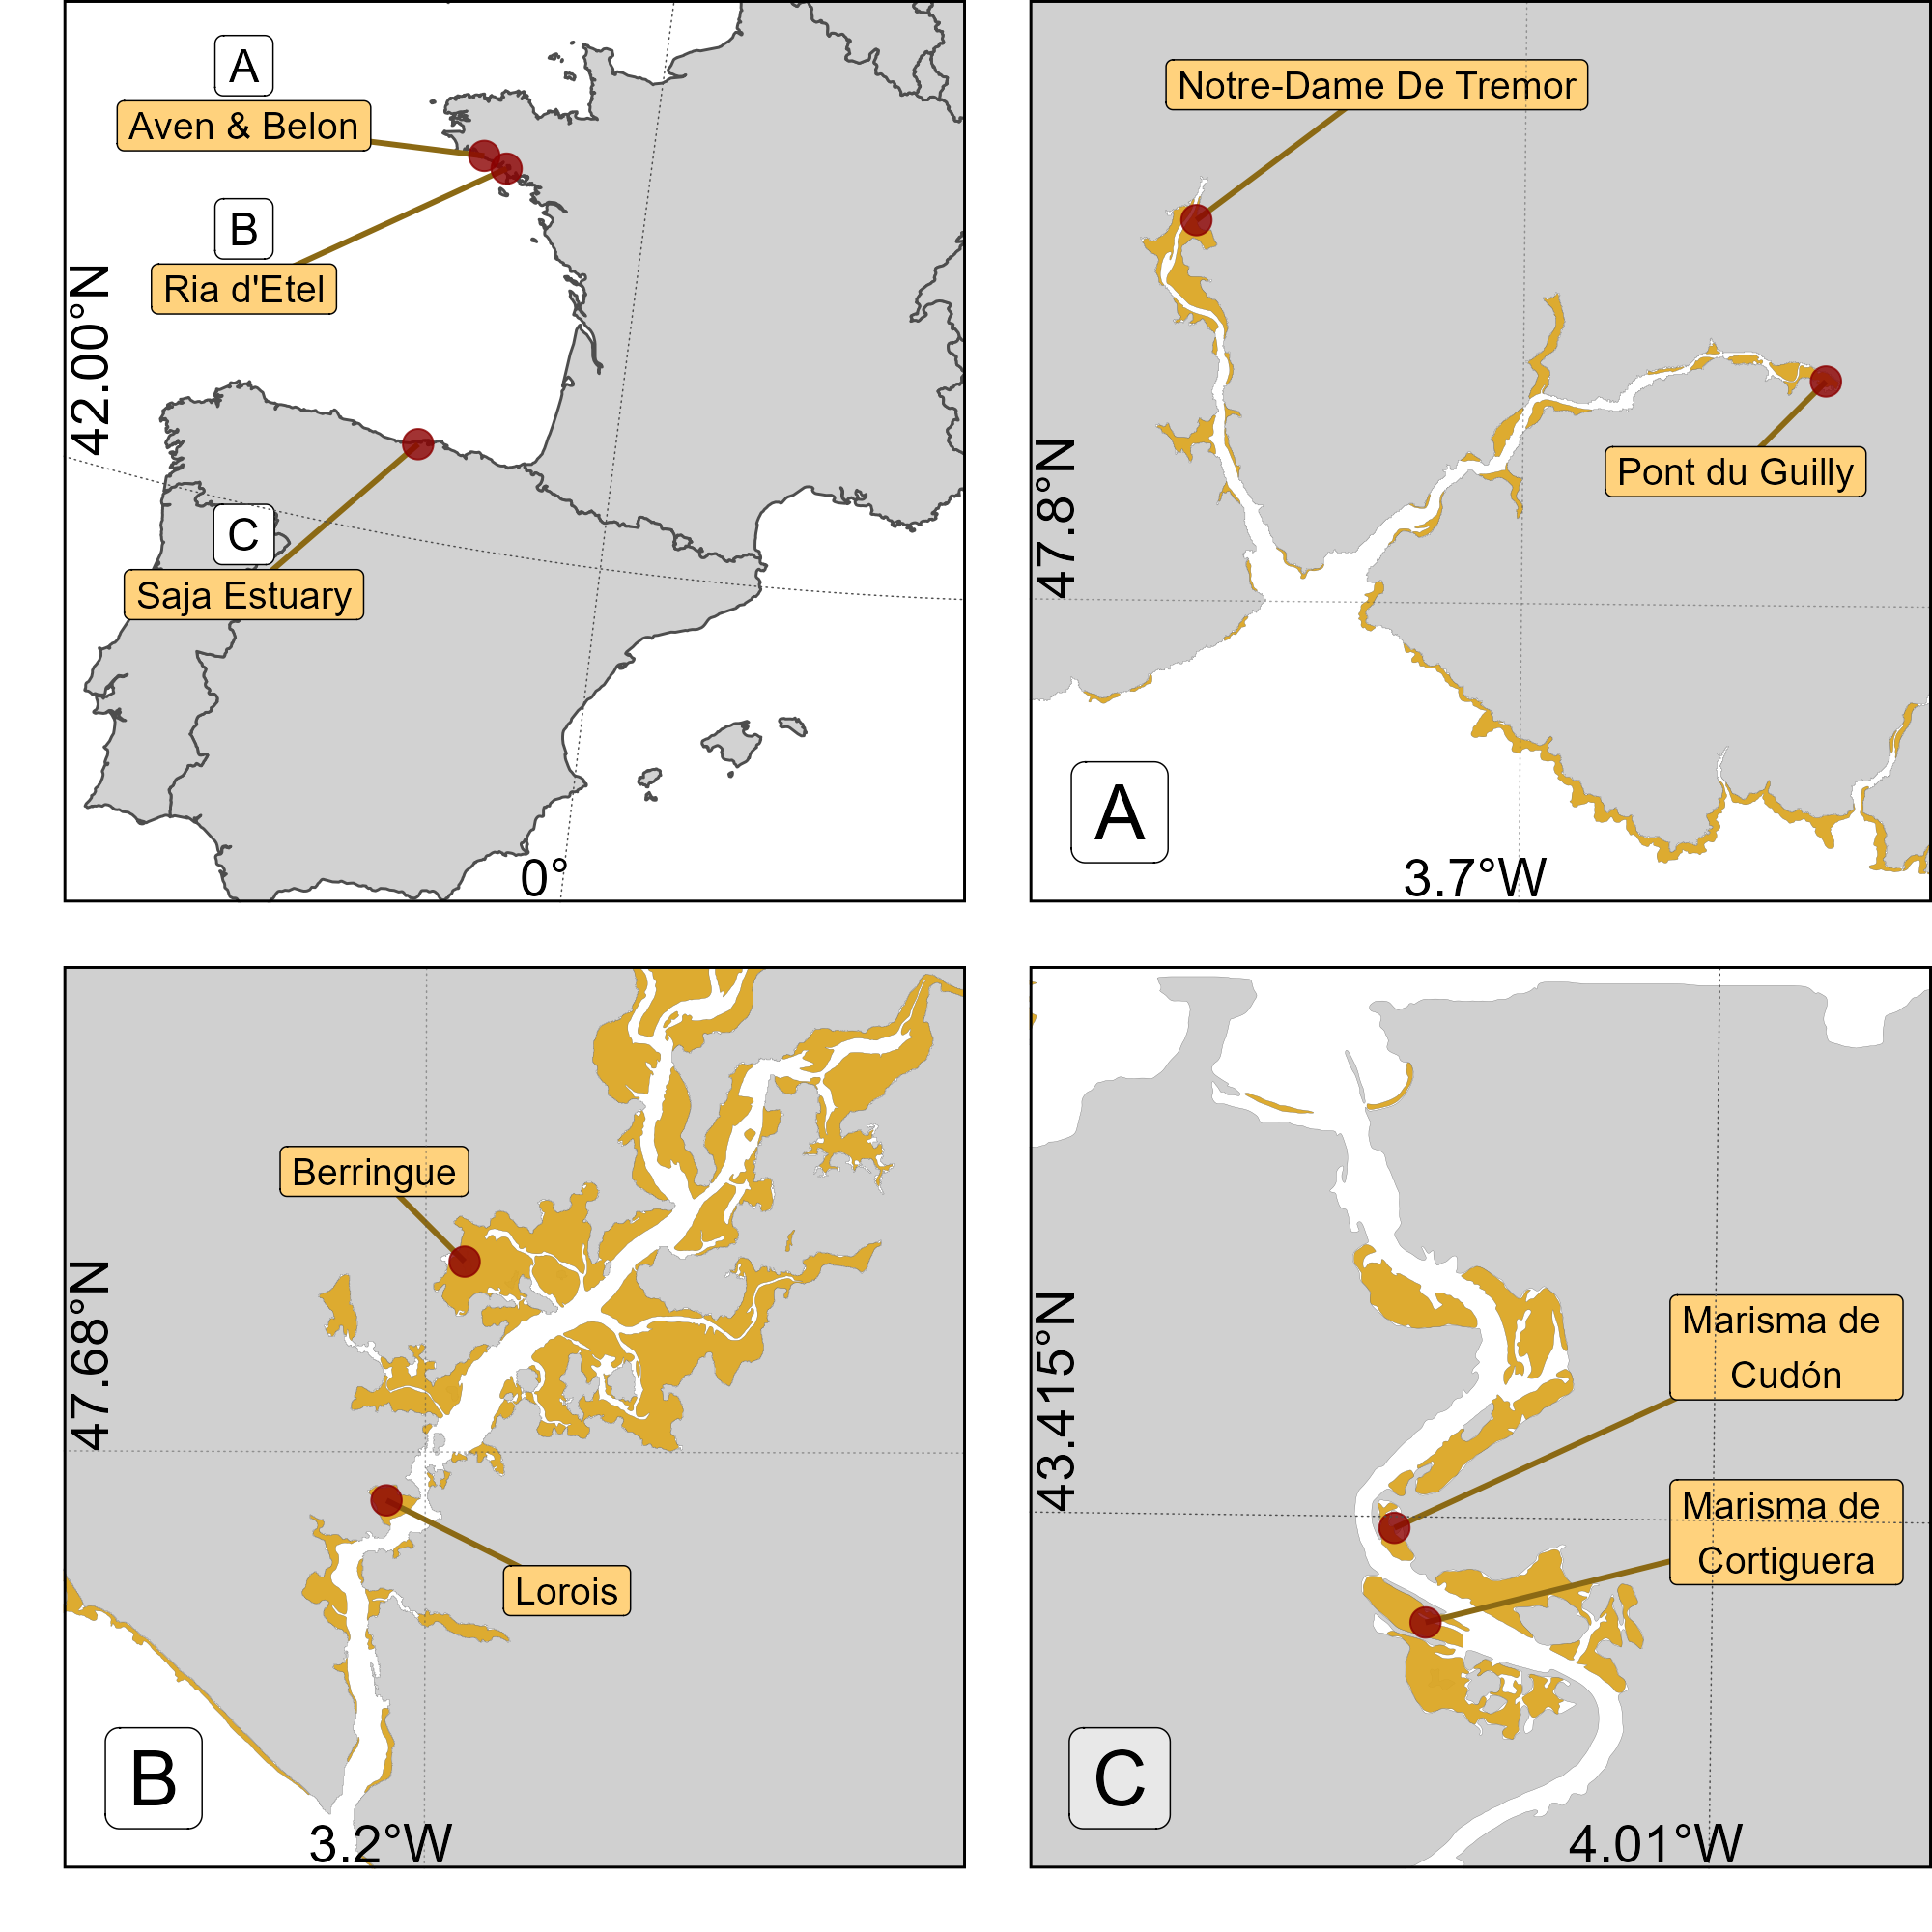
\includegraphics[width=0.95\linewidth,height=\textheight,keepaspectratio]{Figures/Low_res/Figure1/Map_site.png}

}

\caption{\label{fig-location_sites}Location of the drone flights. A:
Flights made in Aven \& Belon Estuaries, France; B: Flights made in Etel
Estuary, France; C: Flights made in Saja Estuaries, Spain. Golden
polygons represent intertidal areas.}

\end{figure}%

\subsection{Drone flights}\label{drone-flights}

\subsubsection{Multispectral data}\label{multispectral-data}

At each location (Table~\ref{tbl-flights}), reflectance images with a
resolution of 1.2 million pixels were captured using a DJI Matrice 300
quadcopter drone equipped with a Micasense RedEdge Dual MX multispectral
camera. The camera recorded data across ten spectral bands, spanning
from blue to near-infrared (NIR) wavelengths (444, 475, 531, 560, 650,
668, 705, 717, 740, and 840 nm) (). To ensure consistent lighting
conditions, the drone's flight trajectory was aligned to maintain a
solar azimuth angle of 90 degrees. Image acquisition was carried out
with an overlap of 70\% between side-by-side images and 80\% between
successive images along the flight path. A downwelling light sensor
(DLS2) was used to measure real-time irradiance, enabling the correction
of reflectance values for variations in light intensity caused by cloud
cover during the flight. The raw image data were subsequently calibrated
to reflectance using a calibration panel with \textasciitilde50\%
reflectivity, provided by the camera's manufacturer. Images were
processed using structure-from-motion photogrammetry software (Agisoft,
2019) to generate multispectral orthomosaics for each flight. The
orthomosaicking workflow was consistent across all flights. Initially,
key tie points were identified within each image and across overlapping
images to create a sparse point cloud. This point cloud was refined by
removing noisy points using a reprojection accuracy metric.
Subsequently, a dense point cloud was generated using a
structure-from-motion algorithm. A digital surface model (DSM) was then
created through surface interpolation of the dense point cloud, which
served as the basis for reconstructing the multispectral ortho-image
(Nebel et al., 2020). The resolution of the multispectral orthomosaic
obtained were 8 cm per pixel.

\subsubsection{LiDAR data}\label{lidar-data}

Using the Matrice 300 Series Dual Gimbal Connector, a DJI Zenmuse L1
LiDAR and RGB sensor was mounted on the drone alongside the
Multispectral camera. This configuration enabled the simultaneous
recording of LiDAR point clouds, high resolution RGB images and
multispectral images captured by the Micasense RedEdge Dual MX during
the same flight. Settings of the LiDAR has been set to have a point
density of 350 m\(^{-2}\)

\begin{table}

\caption{\label{tbl-flights}List of drone flights, summarising the
location, the date, and the total extent of each flight (in hectars).}

\centering{


\includegraphics[width=8.84in,height=\textheight,keepaspectratio]{Figures/High_res/table_flights.png}

}

\end{table}%

\section{Results}\label{results}

\section{Discussion}\label{discussion}

\section{Conclusion}\label{conclusion}

\section*{References}\label{references}
\addcontentsline{toc}{section}{References}

\phantomsection\label{refs}
\begin{CSLReferences}{1}{0}
\bibitem[\citeproctext]{ref-abreu2011nitrogen}
Abreu, M.H., Pereira, R., Buschmann, A., Sousa-Pinto, I., Yarish, C.,
2011. Nitrogen uptake responses of gracilaria vermiculophylla (ohmi)
papenfuss under combined and single addition of nitrate and ammonium.
Journal of Experimental Marine Biology and Ecology 407, 190--199.

\bibitem[\citeproctext]{ref-agisoft}
Agisoft, 2019. \href{https://www.agisoft.com/}{Agisoft metashape}.

\bibitem[\citeproctext]{ref-barbier2011value}
Barbier, E.B., Hacker, S.D., Kennedy, C., Koch, E.W., Stier, A.C.,
Silliman, B.R., 2011. The value of estuarine and coastal ecosystem
services. Ecological monographs 81, 169--193.

\bibitem[\citeproctext]{ref-Blanchet2014}
Blanchet, H., Gouillieux, B., Alizier, S., others, 2014. Multiscale
patterns in the diversity and organization of benthic intertidal fauna
among french atlantic estuaries. Journal of Sea Research 90, 95--110.
\url{https://doi.org/10.1016/j.seares.2014.02.014}

\bibitem[\citeproctext]{ref-capdevila2019warming}
Capdevila, P., Hereu, B., Salguero-Gómez, R., Rovira, G. la, Medrano,
A., Cebrian, E., Garrabou, J., Kersting, D.K., Linares, C., 2019.
Warming impacts on early life stages increase the vulnerability and
delay the population recovery of a long-lived habitat-forming macroalga.
Journal of Ecology 107, 1129--1140.

\bibitem[\citeproctext]{ref-Castaing1995}
Castaing, P., Guilcher, A., 1995. Morphosedimentary evolution of
ria-type estuaries. Earth Surface Processes and Landforms 20, 361--376.
\url{https://doi.org/10.1002/esp.3290200408}

\bibitem[\citeproctext]{ref-Cianfaglione2018}
Cianfaglione, K., 2021. Plant landscape and models of french atlantic
estuarine systems: Extended summary of the doctoral thesis.
Transylvanian Review of Systematical and Ecological Research 23, 15--36.
\url{https://doi.org/10.2478/trser-2021-0002}

\bibitem[\citeproctext]{ref-davies2024sentinel}
Davies, B.F.R., Oiry, S., Rosa, P., Zoffoli, M.L., Sousa, A.I., Thomas,
O.R., Smale, D.A., Austen, M.C., Biermann, L., Attrill, M.J., others,
2024b. A sentinel watching over inter-tidal seagrass phenology across
western europe and north africa. Communications Earth \& Environment 5,
382.

\bibitem[\citeproctext]{ref-davies2024intertidal}
Davies, B.F.R., Oiry, S., Rosa, P., Zoffoli, M.L., Sousa, A.I., Thomas,
O.R., Smale, D.A., Austen, M.C., Biermann, L., Attrill, M.J., others,
2024a. Intertidal seagrass extent from sentinel-2 time-series show
distinct trajectories in western europe. Remote Sensing of Environment
312, 114340.

\bibitem[\citeproctext]{ref-de2023valuing}
De Valck, J., Jarvis, D., Coggan, A., Schirru, E., Pert, P., Graham, V.,
Newlands, M., 2023. Valuing ecosystem services in complex coastal
settings: An extended ecosystem accounting framework for improved
decision-making. Marine Policy 155, 105761.

\bibitem[\citeproctext]{ref-Gentric2024}
Gentric, C., Sauleau, P., 2024. Bacterial load mitigation of the
shellfish magallana gigas by the marine sponge hymeniacidon perlevis
(montagu 1818). Regional Studies in Marine Science 75, 103564.
\url{https://doi.org/10.1016/j.rsma.2024.103564}

\bibitem[\citeproctext]{ref-van2018global}
Ginneken, V. van, Vries, E. de, others, 2018. The global dispersal of
the non-endemic invasive red alga gracilaria vermiculophylla in the
ecosystems of the euro-asia coastal waters including the wadden sea
unesco world heritage coastal area: Awful or awesome? Oceanography \&
Fisheries Open Access Journal 8, 4--26.

\bibitem[\citeproctext]{ref-hall2019ocean}
Hall-Spencer, J.M., Harvey, B.P., 2019. Ocean acidification impacts on
coastal ecosystem services due to habitat degradation. Emerging Topics
in Life Sciences 3, 197--206.

\bibitem[\citeproctext]{ref-he2019climate}
He, Q., Silliman, B.R., 2019. Climate change, human impacts, and coastal
ecosystems in the anthropocene. Current Biology 29, R1021--R1035.

\bibitem[\citeproctext]{ref-Jeanneau2023}
Jeanneau, L., Jardé, E., Louis, J., Pannard, A., Liotaud, M.,
Andrieux-Loyer, F., Gruau, G., Caradec, F., Rabiller, E., Lebris, N.,
Laverman, A., 2023. How the origin of sedimentary organic matter impacts
the benthic nutrient fluxes in shallow coastal mudflats. Comptes Rendus
Géoscience 355, 237--258. \url{https://doi.org/10.5802/crgeos.228}

\bibitem[\citeproctext]{ref-krueger2018everywhere}
Krueger-Hadfield, S., 2018. Everywhere you look, everywhere you go,
there's an estuary invaded by the red seaweed gracilaria vermiculophylla
(ohmi) papenfuss, 1967. BioInvasions Records 7.

\bibitem[\citeproctext]{ref-krueger2017genetic}
Krueger-Hadfield, S.A., Kollars, N.M., Strand, A.E., Byers, J.E.,
Shainker, S.J., Terada, R., Greig, T.W., Hammann, M., Murray, D.C.,
Weinberger, F., others, 2017. Genetic identification of source and
likely vector of a widespread marine invader. Ecology and evolution 7,
4432--4447.

\bibitem[\citeproctext]{ref-liquete2013current}
Liquete, C., Piroddi, C., Drakou, E.G., Gurney, L., Katsanevakis, S.,
Charef, A., Egoh, B., 2013. Current status and future prospects for the
assessment of marine and coastal ecosystem services: A systematic
review. PloS one 8, e67737.

\bibitem[\citeproctext]{ref-liu2020ocean}
Liu, C., Zou, D., Liu, Z., Ye, C., 2020. Ocean warming alters the
responses to eutrophication in a commercially farmed seaweed,
gracilariopsis lemaneiformis. Hydrobiologia 847, 879--893.

\bibitem[\citeproctext]{ref-lu2018major}
Lu, Y., Yuan, J., Lu, X., Su, C., Zhang, Y., Wang, C., Cao, X., Li, Q.,
Su, J., Ittekkot, V., others, 2018. Major threats of pollution and
climate change to global coastal ecosystems and enhanced management for
sustainability. Environmental Pollution 239, 670--680.

\bibitem[\citeproctext]{ref-mehvar2018quantifying}
Mehvar, S., Filatova, T., Dastgheib, A., De Ruyter van Steveninck, E.,
Ranasinghe, R., 2018. Quantifying economic value of coastal ecosystem
services: A review. Journal of marine science and engineering 6, 5.

\bibitem[\citeproctext]{ref-Michel2021}
Michel, G., Le Bot, S., Lesourd, S., Lafite, R., 2021.
Morpho-sedimentological and dynamic patterns in a ria type estuary: The
belon estuary (south brittany, france). Journal of Maps 17, 389--400.
\url{https://doi.org/10.1080/17445647.2021.1925170}

\bibitem[\citeproctext]{ref-mukherjee2023coastal}
Mukherjee, S., Ghosh, K.K., Chanda, A., 2023. Coastal pollution---an
overview. Environmental Oceanography and Coastal Dynamics: Current
Scenario and Future Trends 99--107.

\bibitem[\citeproctext]{ref-nebel2020review}
Nebel, S., Beege, M., Schneider, S., Rey, G.D., 2020. A review of
photogrammetry and photorealistic 3D models in education from a
psychological perspective, in: Frontiers in Education. Frontiers Media
SA, p. 144.

\bibitem[\citeproctext]{ref-nyberg2009flora}
Nyberg, C.D., Thomsen, M.S., Wallentinus, I., 2009. Flora and fauna
associated with the introduced red alga gracilaria vermiculophylla.
European Journal of Phycology 44, 395--403.

\bibitem[\citeproctext]{ref-ortega2005fluxes}
Ortega, T., Ponce, R., Forja, J., Gómez-Parra, A., 2005. Fluxes of
dissolved inorganic carbon in three estuarine systems of the cantabrian
sea (north of spain). Journal of Marine Systems 53, 125--142.

\bibitem[\citeproctext]{ref-Portas2023}
Portas, A., Carriot, N., Ortalo-Magné, A., Damblans, G., Thiébaut, M.,
Culioli, G., Quillien, N., Briand, J.-F., 2023. Impact of hydrodynamics
on community structure and metabolic production of marine biofouling
formed in a highly energetic estuary. Marine Environmental Research 192,
106241. \url{https://doi.org/10.1016/j.marenvres.2023.106241}

\bibitem[\citeproctext]{ref-ramus2017invasive}
Ramus, A.P., Silliman, B.R., Thomsen, M.S., Long, Z.T., 2017. An
invasive foundation species enhances multifunctionality in a coastal
ecosystem. Proceedings of the national academy of sciences 114,
8580--8585.

\bibitem[\citeproctext]{ref-roman2024mapping}
Román, A., Oiry, S., Davies, B.F., Rosa, P., Gernez, P., Tovar-Sánchez,
A., Navarro, G., Méléder, V., Barillé, L., 2024. Mapping intertidal
microphytobenthic biomass with very high-resolution remote sensing
imagery in an estuarine system. Science of The Total Environment 177025.

\bibitem[\citeproctext]{ref-roman2023mapping}
Román, A., Prasyad, H., Oiry, S., Davies, B.F., Brunier, G., Barillé,
L., 2023. Mapping intertidal oyster farms using unmanned aerial vehicles
(UAV) high-resolution multispectral data. Estuarine, Coastal and Shelf
Science 291, 108432.

\bibitem[\citeproctext]{ref-roman2021using}
Román, A., Tovar-Sánchez, A., Olivé, I., Navarro, G., 2021. Using a
UAV-mounted multispectral camera for the monitoring of marine
macrophytes. Frontiers in Marine Science 8, 722698.

\bibitem[\citeproctext]{ref-romero2008sintering}
Romero, M., Andrés, A., Alonso, R., Viguri, J., Rincón, J.M., 2008.
Sintering behaviour of ceramic bodies from contaminated marine
sediments. Ceramics International 34, 1917--1924.

\bibitem[\citeproctext]{ref-rueness2005life}
Rueness, J., 2005. Life history and molecular sequences of gracilaria
vermiculophylla (gracilariales, rhodophyta), a new introduction to
european waters. Phycologia 44, 120--128.

\bibitem[\citeproctext]{ref-seitz2014ecological}
Seitz, R.D., Wennhage, H., Bergström, U., Lipcius, R.N., Ysebaert, T.,
2014. Ecological value of coastal habitats for commercially and
ecologically important species. ICES Journal of Marine Science 71,
648--665.

\bibitem[\citeproctext]{ref-small2003global}
Small, C., Nicholls, R.J., 2003. A global analysis of human settlement
in coastal zones. Journal of coastal research 584--599.

\bibitem[\citeproctext]{ref-sotka2018combining}
Sotka, E.E., Baumgardner, A.W., Bippus, P.M., Destombe, C., Duermit,
E.A., Endo, H., Flanagan, B.A., Kamiya, M., Lees, L.E., Murren, C.J.,
others, 2018. Combining niche shift and population genetic analyses
predicts rapid phenotypic evolution during invasion. Evolutionary
Applications 11, 781--793.

\bibitem[\citeproctext]{ref-Tankoua2011}
Tankoua, O.F., Buffet, P.-E., Amiard, J.-C., Amiard-Triquet, C.,
Mouneyrac, C., Berthet, B., 2011. Potential influence of confounding
factors (size, salinity) on biomarkers in the sentinel species
scrobicularia plana used in programmes monitoring estuarine quality.
Environmental Science and Pollution Research 18, 1253--1263.
\url{https://doi.org/10.1007/s11356-011-0479-3}

\bibitem[\citeproctext]{ref-thomsen2013effects}
Thomsen, M.S., Stæhr, P.A., Nejrup, L., Schiel, D.R., 2013. Effects of
the invasive macroalgae gracilaria vermiculophylla on two co-occurring
foundation species and associated invertebrates. Aquatic Invasions 8,
133--145.

\bibitem[\citeproctext]{ref-unsworth2022planetary}
Unsworth, R.K., Cullen-Unsworth, L.C., Jones, B.L., Lilley, R.J., 2022.
The planetary role of seagrass conservation. Science 377, 609--613.

\bibitem[\citeproctext]{ref-van2003reintroduction}
Van Katwijk, M., 2003. Reintroduction of eelgrass (zostera marina l.) in
the dutch wadden sea: A research overview and management vision, in:
Challenges to the Wadden Sea Area. In: Proceedings of the 10th
International Scientific Wadden Sea Symposium, Groningen, the
Netherlands. pp. 173--195.

\bibitem[\citeproctext]{ref-watanabe2018introduction}
Watanabe, Y., Kawamura, T., Yamashita, Y., 2018. Introduction: The
coastal ecosystem complex as a unit of structure and function of
biological productivity in coastal areas. Fisheries science 84,
149--152.

\bibitem[\citeproctext]{ref-weinberger2008invasive}
Weinberger, F., Buchholz, B., Karez, R., Wahl, M., 2008. The invasive
red alga gracilaria vermiculophylla in the baltic sea: Adaptation to
brackish water may compensate for light limitation. Aquatic Biology 3,
251--264.

\bibitem[\citeproctext]{ref-zoffoli2021decadal}
Zoffoli, M.L., Gernez, P., Godet, L., Peters, S., Oiry, S., Barillé, L.,
2021. Decadal increase in the ecological status of a north-atlantic
intertidal seagrass meadow observed with multi-mission satellite
time-series. Ecological Indicators 130, 108033.

\end{CSLReferences}




\end{document}
